\documentclass[a4paper]{article}

%====================== PACKAGES ======================

\usepackage[french]{babel}
\usepackage[utf8x]{inputenc}
%pour gérer les positionnement d'images
\usepackage{float}
\usepackage{amsmath}
\usepackage{graphicx}
\usepackage[colorinlistoftodos]{todonotes}
\usepackage{url}
%pour les informations sur un document compilé en PDF et les liens externes / internes
\usepackage{hyperref}
%pour la mise en page des tableaux
\usepackage{array}
\usepackage{tabularx}
%pour utiliser \floatbarrier
%\usepackage{placeins}
%\usepackage{floatrow}
%espacement entre les lignes
\usepackage{setspace}
%modifier la mise en page de l'abstract
\usepackage{abstract}
%police et mise en page (marges) du document
\usepackage[T1]{fontenc}
\usepackage[top=2cm, bottom=2cm, left=2cm, right=2cm]{geometry}
%Pour les galerie d'images
\usepackage{subfig}

%====================== INFORMATION ET REGLES ======================

%rajouter les numérotation pour les \paragraphe et \subparagraphe
\setcounter{secnumdepth}{4}
\setcounter{tocdepth}{4}

%======================== DEBUT DU DOCUMENT ========================

\begin{document}

%régler l'espacement entre les lignes
\newcommand{\HRule}{\rule{\linewidth}{0.5mm}}

%page de garde
\begin{titlepage}
\begin{center}

% Upper part of the page. The '~' is needed because only works if a paragraph has started.

\includegraphics[width=0.35\textwidth]{./logo}~\\[2cm]

\vspace{3cm}

\textsc{\LARGE INSA Lyon}\\[0.5cm]
\textsc{\Large Département Informatique}\\[0.5cm]

% Title
\HRule \\[0.4cm]

{\huge \bfseries PLD AGILE : Optimod'Lyon\\
 Rapport de fin de projet\\[0.4cm] }

\HRule \\[1.5cm]

% Author and supervisor
\begin{minipage}{0.4\textwidth}
\begin{flushleft} \large
\emph{Auteur:} H4302\\
Hazim \textsc{Asri}\\
Nihal \textsc{Boutadghart}\\
Jassir \textsc{Habba}\\
Ana \textsc{Martin}\\
Junior \textsc{Noukam}\\
Simon \textsc{Perret}\\
\end{flushleft}
\end{minipage}
\begin{minipage}{0.4\textwidth}
\begin{flushright} \large
\emph{Professeur:} \\
Mme. \textsc{Laforest}\\
\end{flushright}
\end{minipage}

\vfill

% Bottom of the page
{\large \today}

\end{center}
\end{titlepage}

~
%ne pas numéroter cette page
\thispagestyle{empty}

\tableofcontents
\thispagestyle{empty}
\setcounter{page}{0}
%ne pas numéroter le sommaire

%espacement entre les lignes d'un tableau
\renewcommand{\arraystretch}{1.5}

%====================== INCLUSION DES PARTIES ======================

~
\thispagestyle{empty}
%recommencer la numérotation des pages à "1"
\setcounter{page}{0}
\newpage

\section*{Introduction} \label{ch1}

Ce document constitue le livrable de la première itération de notre projet, qui correspond à la phase de démarrache selon la méthodologie USDP (Unified Software Development Process). L'objectif principal de cette phase est de poser les bases de l'application en identifiant les cas d'utilisation majeurs, en concevant une première architecture, et en mettant en œuvre un ensemble limité de cas d'utilisation pour aboutir au MVP, une premiere version limitée mais fonctionnel.\\
\newline
\indent Au cours de cette itération, nous avons concentré nos efforts sur le glossaire, les différents diagrammes tels que le diagramme des cas d'utilisation, le diagramme de classe et package, la mise en place du serveur git, le MVP et encore la documentation. \\
\newline
Le résultat de cette itération est un MVP (Minimum Viable Product) accompagné d'un livrable pour illustrer les avancées réalisées. Ces livrables incluent des diagrammes UML détaillant la conception, une documentation claire des choix architecturaux effectués, ainsi qu’un README structuré pour orienter les utilisateurs et les contributeurs.

\section{Glossaire}

\begin{itemize}
    \item \textbf{Coord} : Représente une paire de coordonnées géographiques (latitude et longitude). Elles fournissent des informations géographiques pour localiser les intersections.
    \item \textbf{Adjacent} : Modélise une connexion entre deux intersections et permet de modéliser le réseau routier.
    \item \textbf{Intersection} : Représente un point du réseau routier, identifié par ses coordonnées géographiques. Sert de noeud dans le réseau routier.
    \item \textbf{Map} : Représente la carte complète du réseau routier et fournit une vue d’ensemble du réseau routier.
    \item \textbf{DeliveryRequest} : Modélise une demande de livraison avec des points de collecte et de livraison. Structure les informations nécessaires à une livraison.
    \item \textbf{Warehouse} : Représente un entrepôt dans le système. Point central pour les départs des tournées.
    \item \textbf{TourRequest} : Regroupe une liste de demandes de livraison associée à un entrepôt. Prépare et organise les demandes de livraison pour une tournée.
    \item \textbf{Courier} : Modélise un livreur.
    \item \textbf{Tour} : Définit une tournée complète incluant plusieurs points d’intersections.   
\end{itemize}

\section{Diagrammes UML}

\subsection{Diagramme des cas d'utilisation}

\begin{figure}[H]
    \centering
    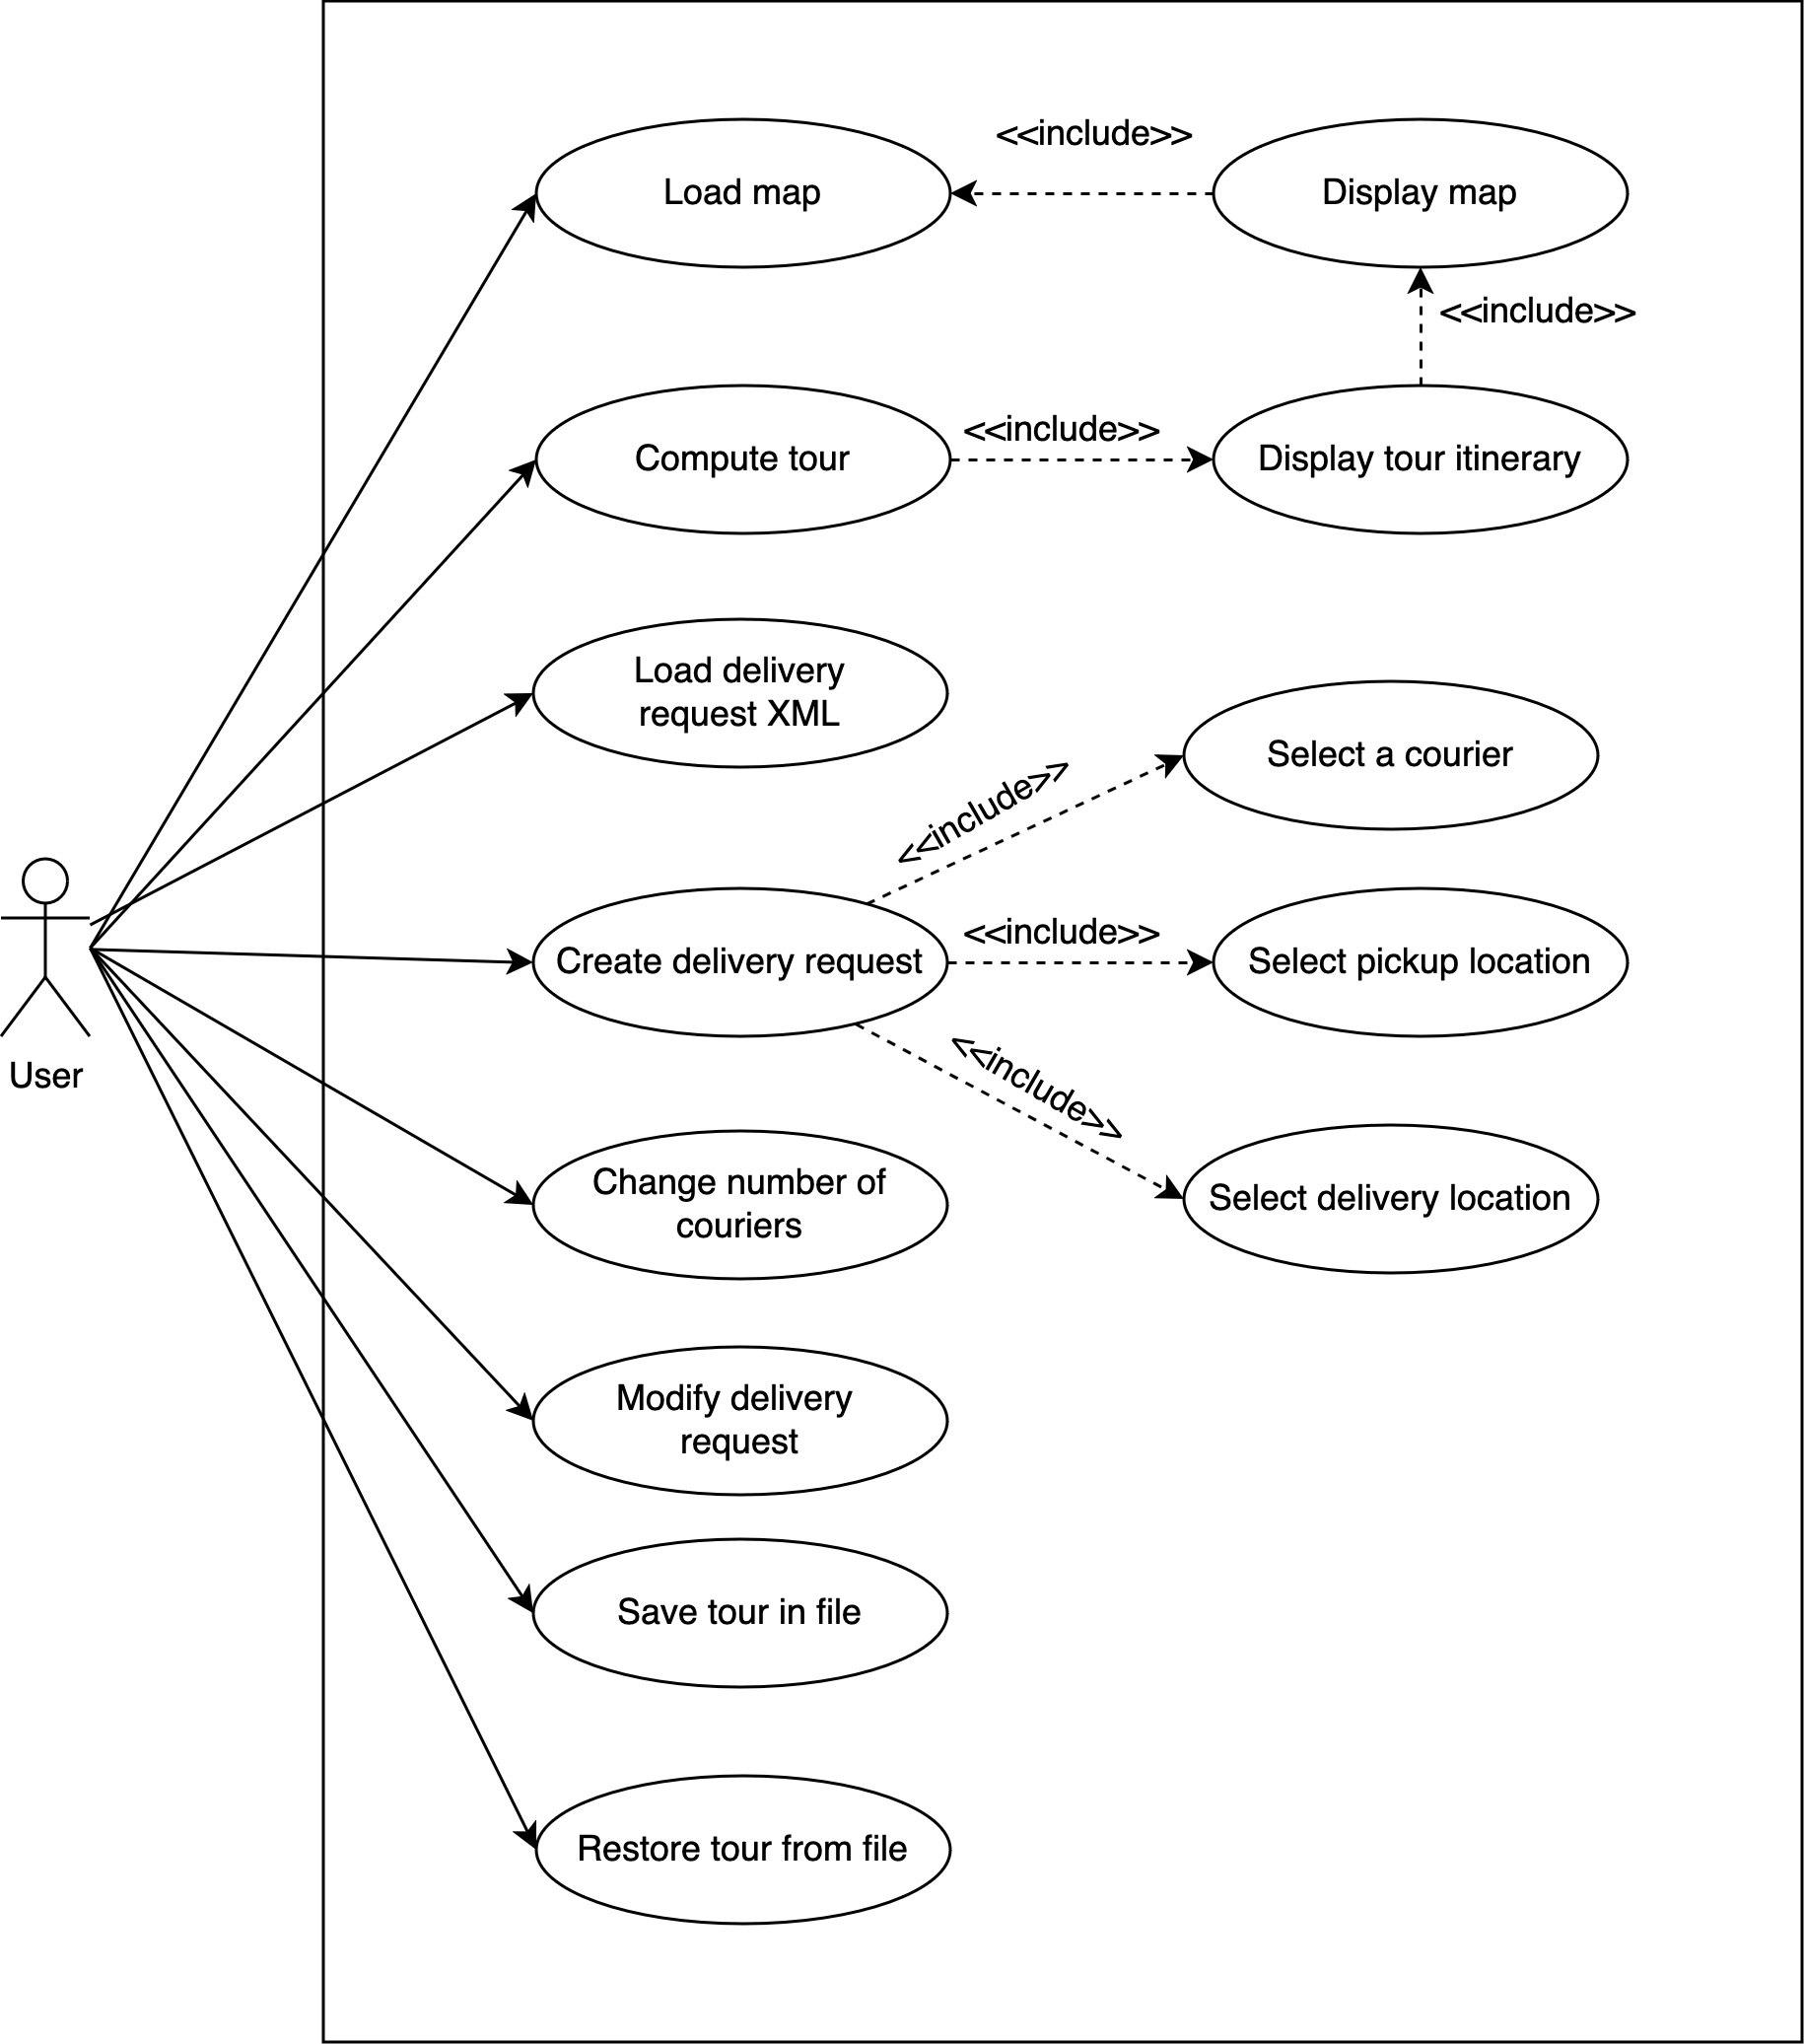
\includegraphics[width=0.75\linewidth]{images/usercase.png}
    \caption{Diagramme des cas d'utilisation}
\end{figure}


\subsection{Diagramme de classe}

\begin{figure}[H]
    \centering
    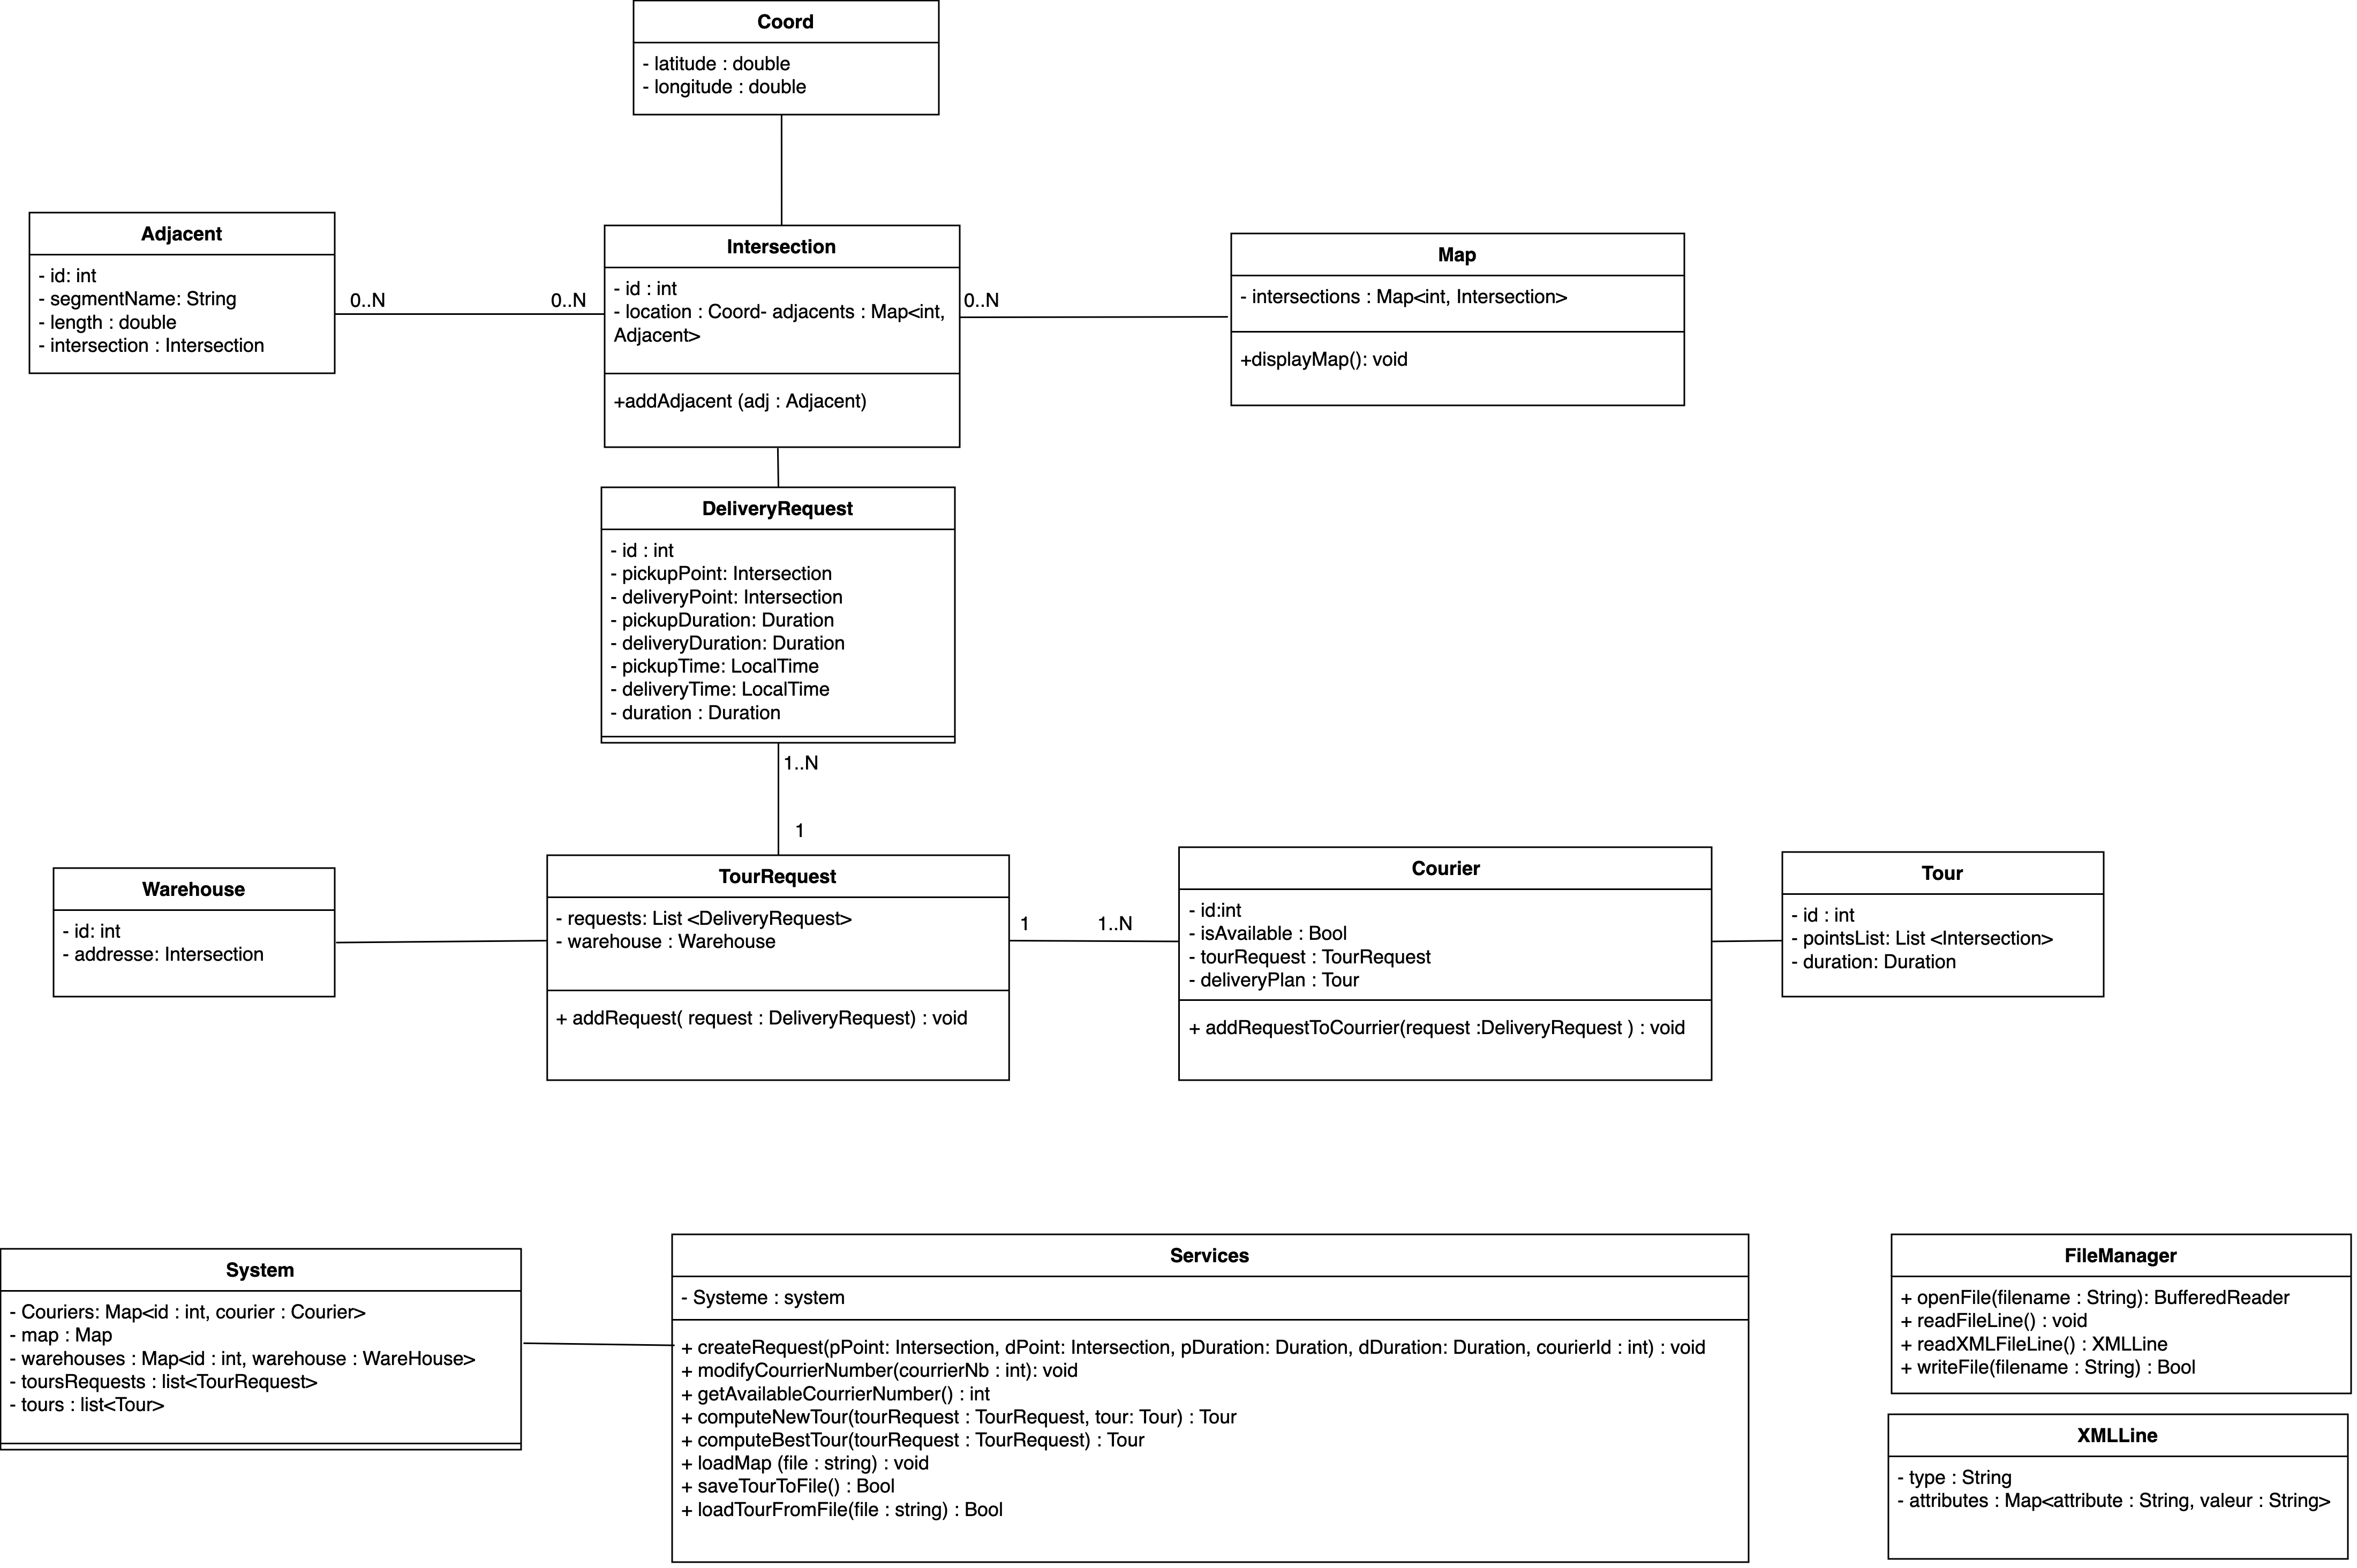
\includegraphics[width=1.2\linewidth, angle=270]{images/class.png}
    \caption{Diagramme de classe}
\end{figure}

\subsection{Package de classe}

\subsection{Diagramme de séquence}

\begin{figure}[H]
    \centering
    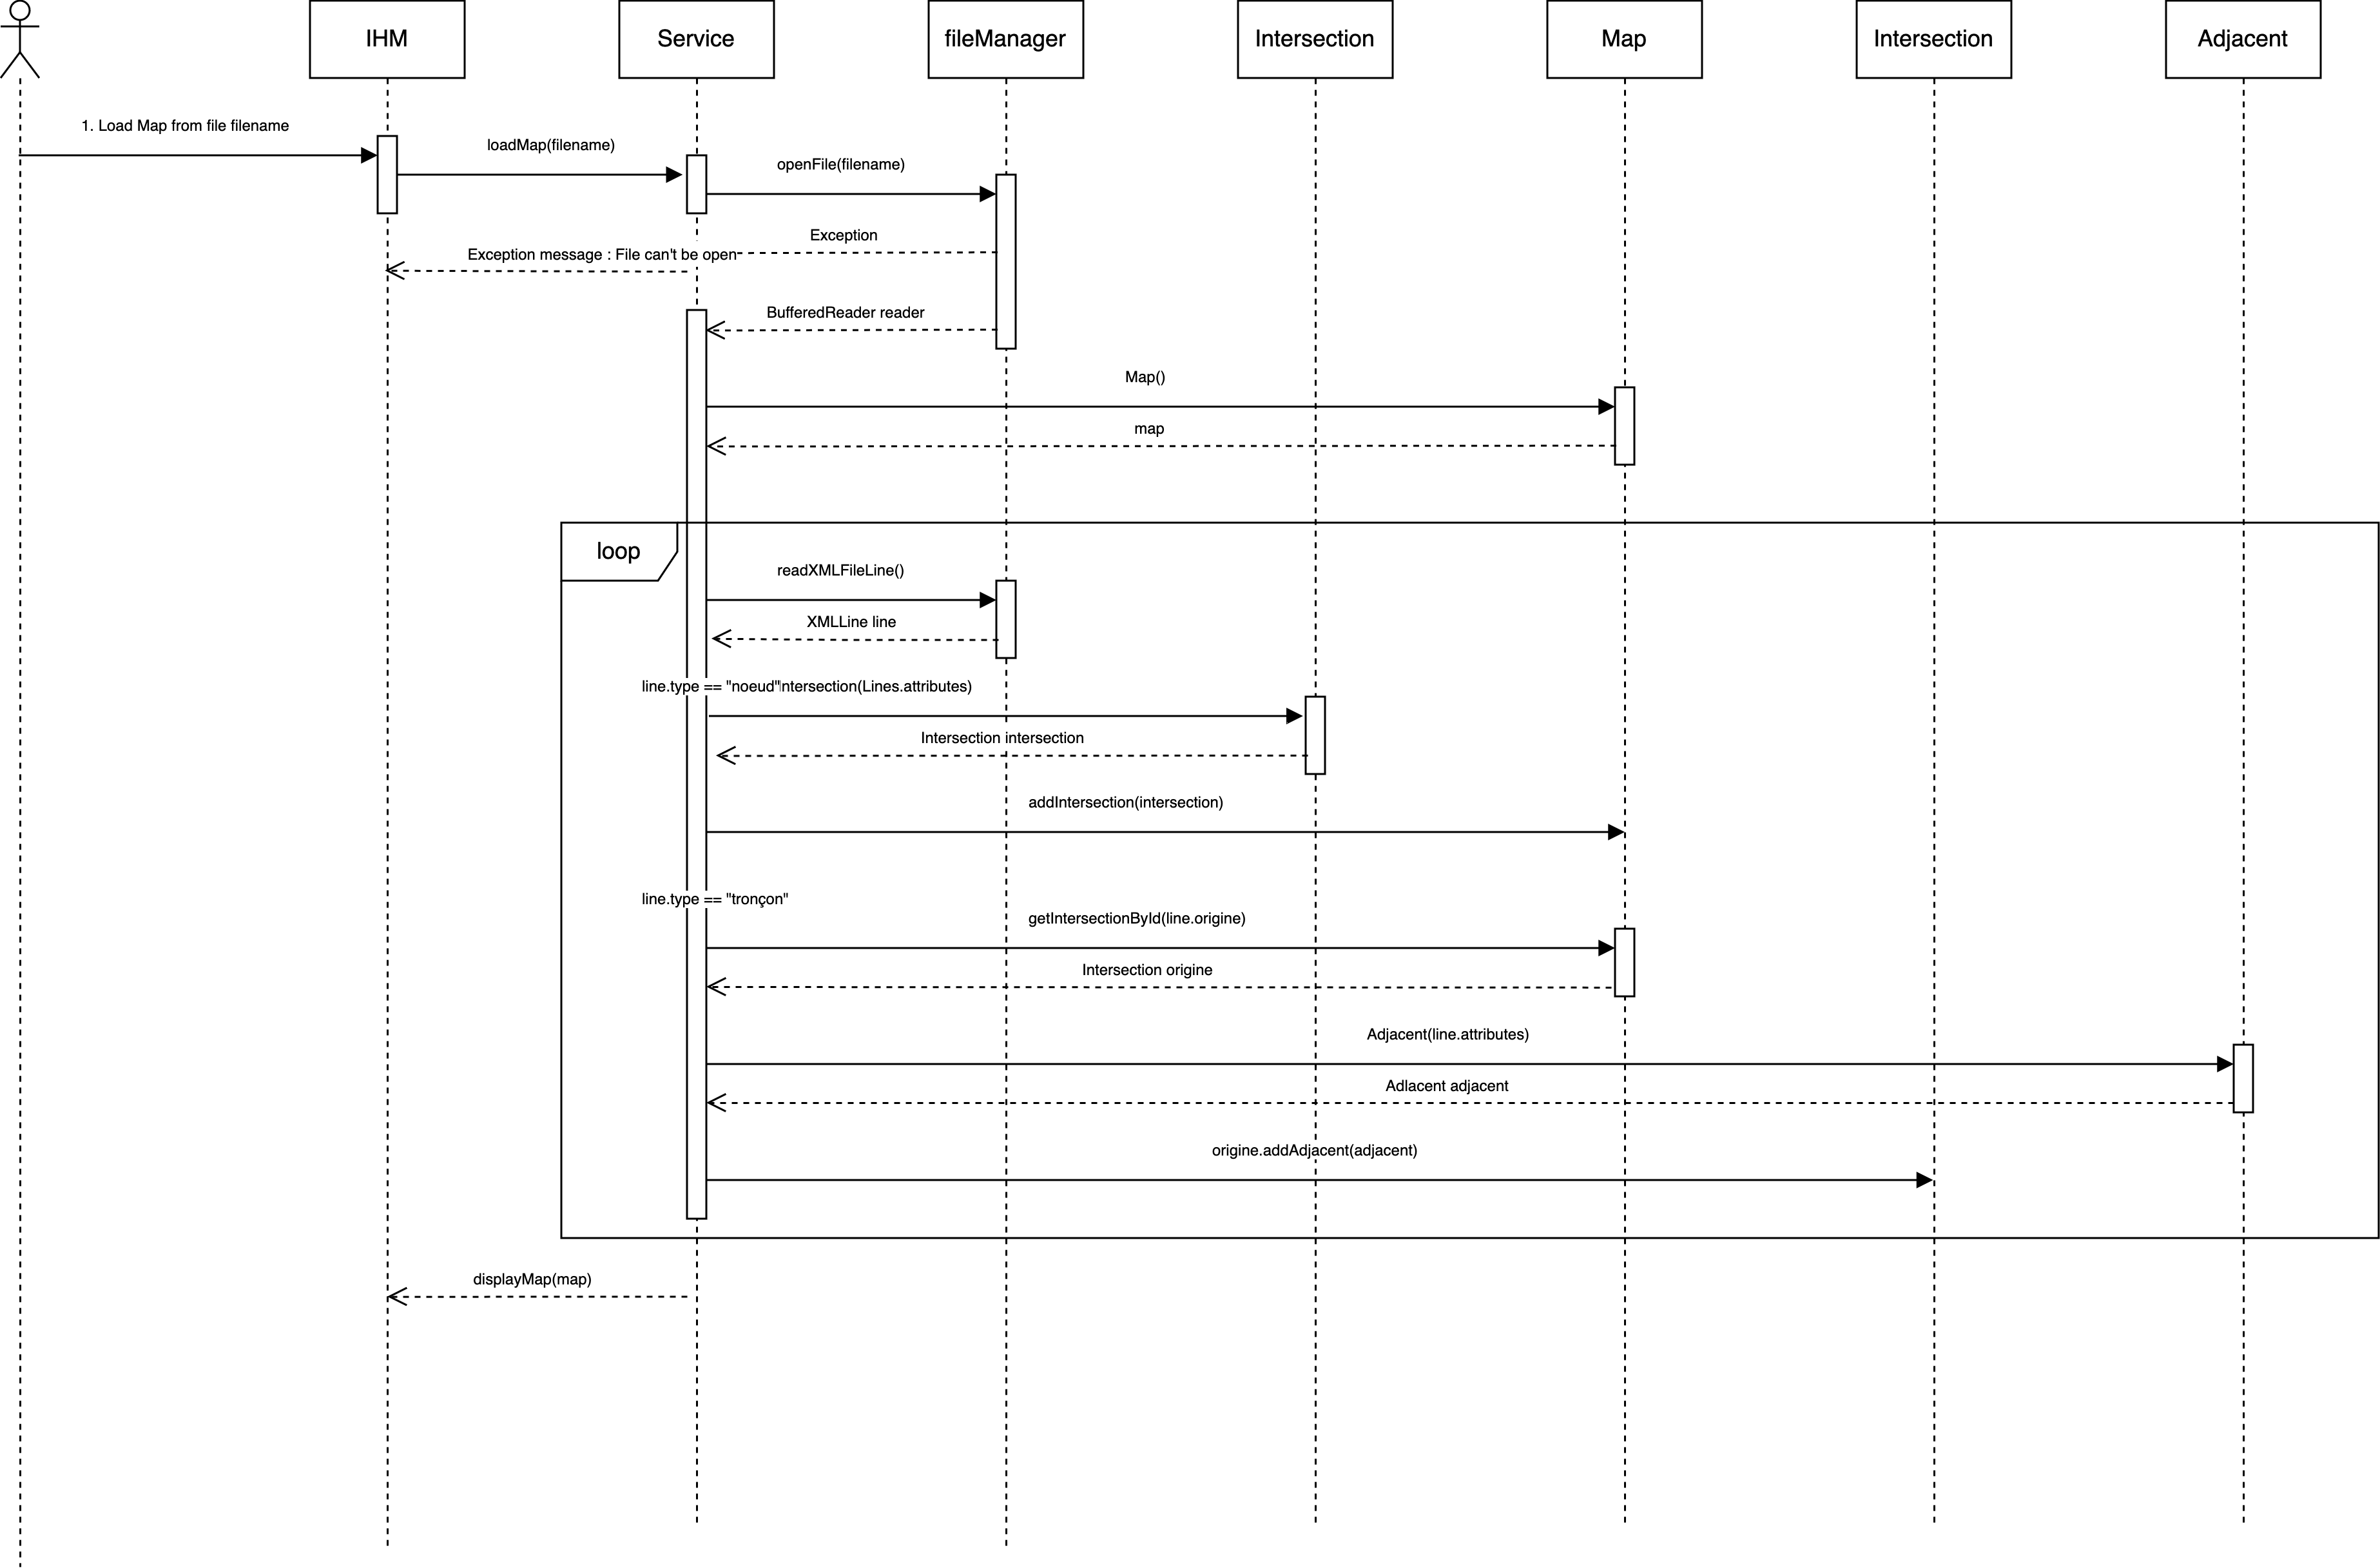
\includegraphics[width=1.15\linewidth, angle=270]{images/sequence-loadmap.png}
    \caption{Diagramme de séquence pour chargement de carte}
\end{figure}

% \section{Design}

\section{Architecture}

\begin{figure}[H]
    \centering
    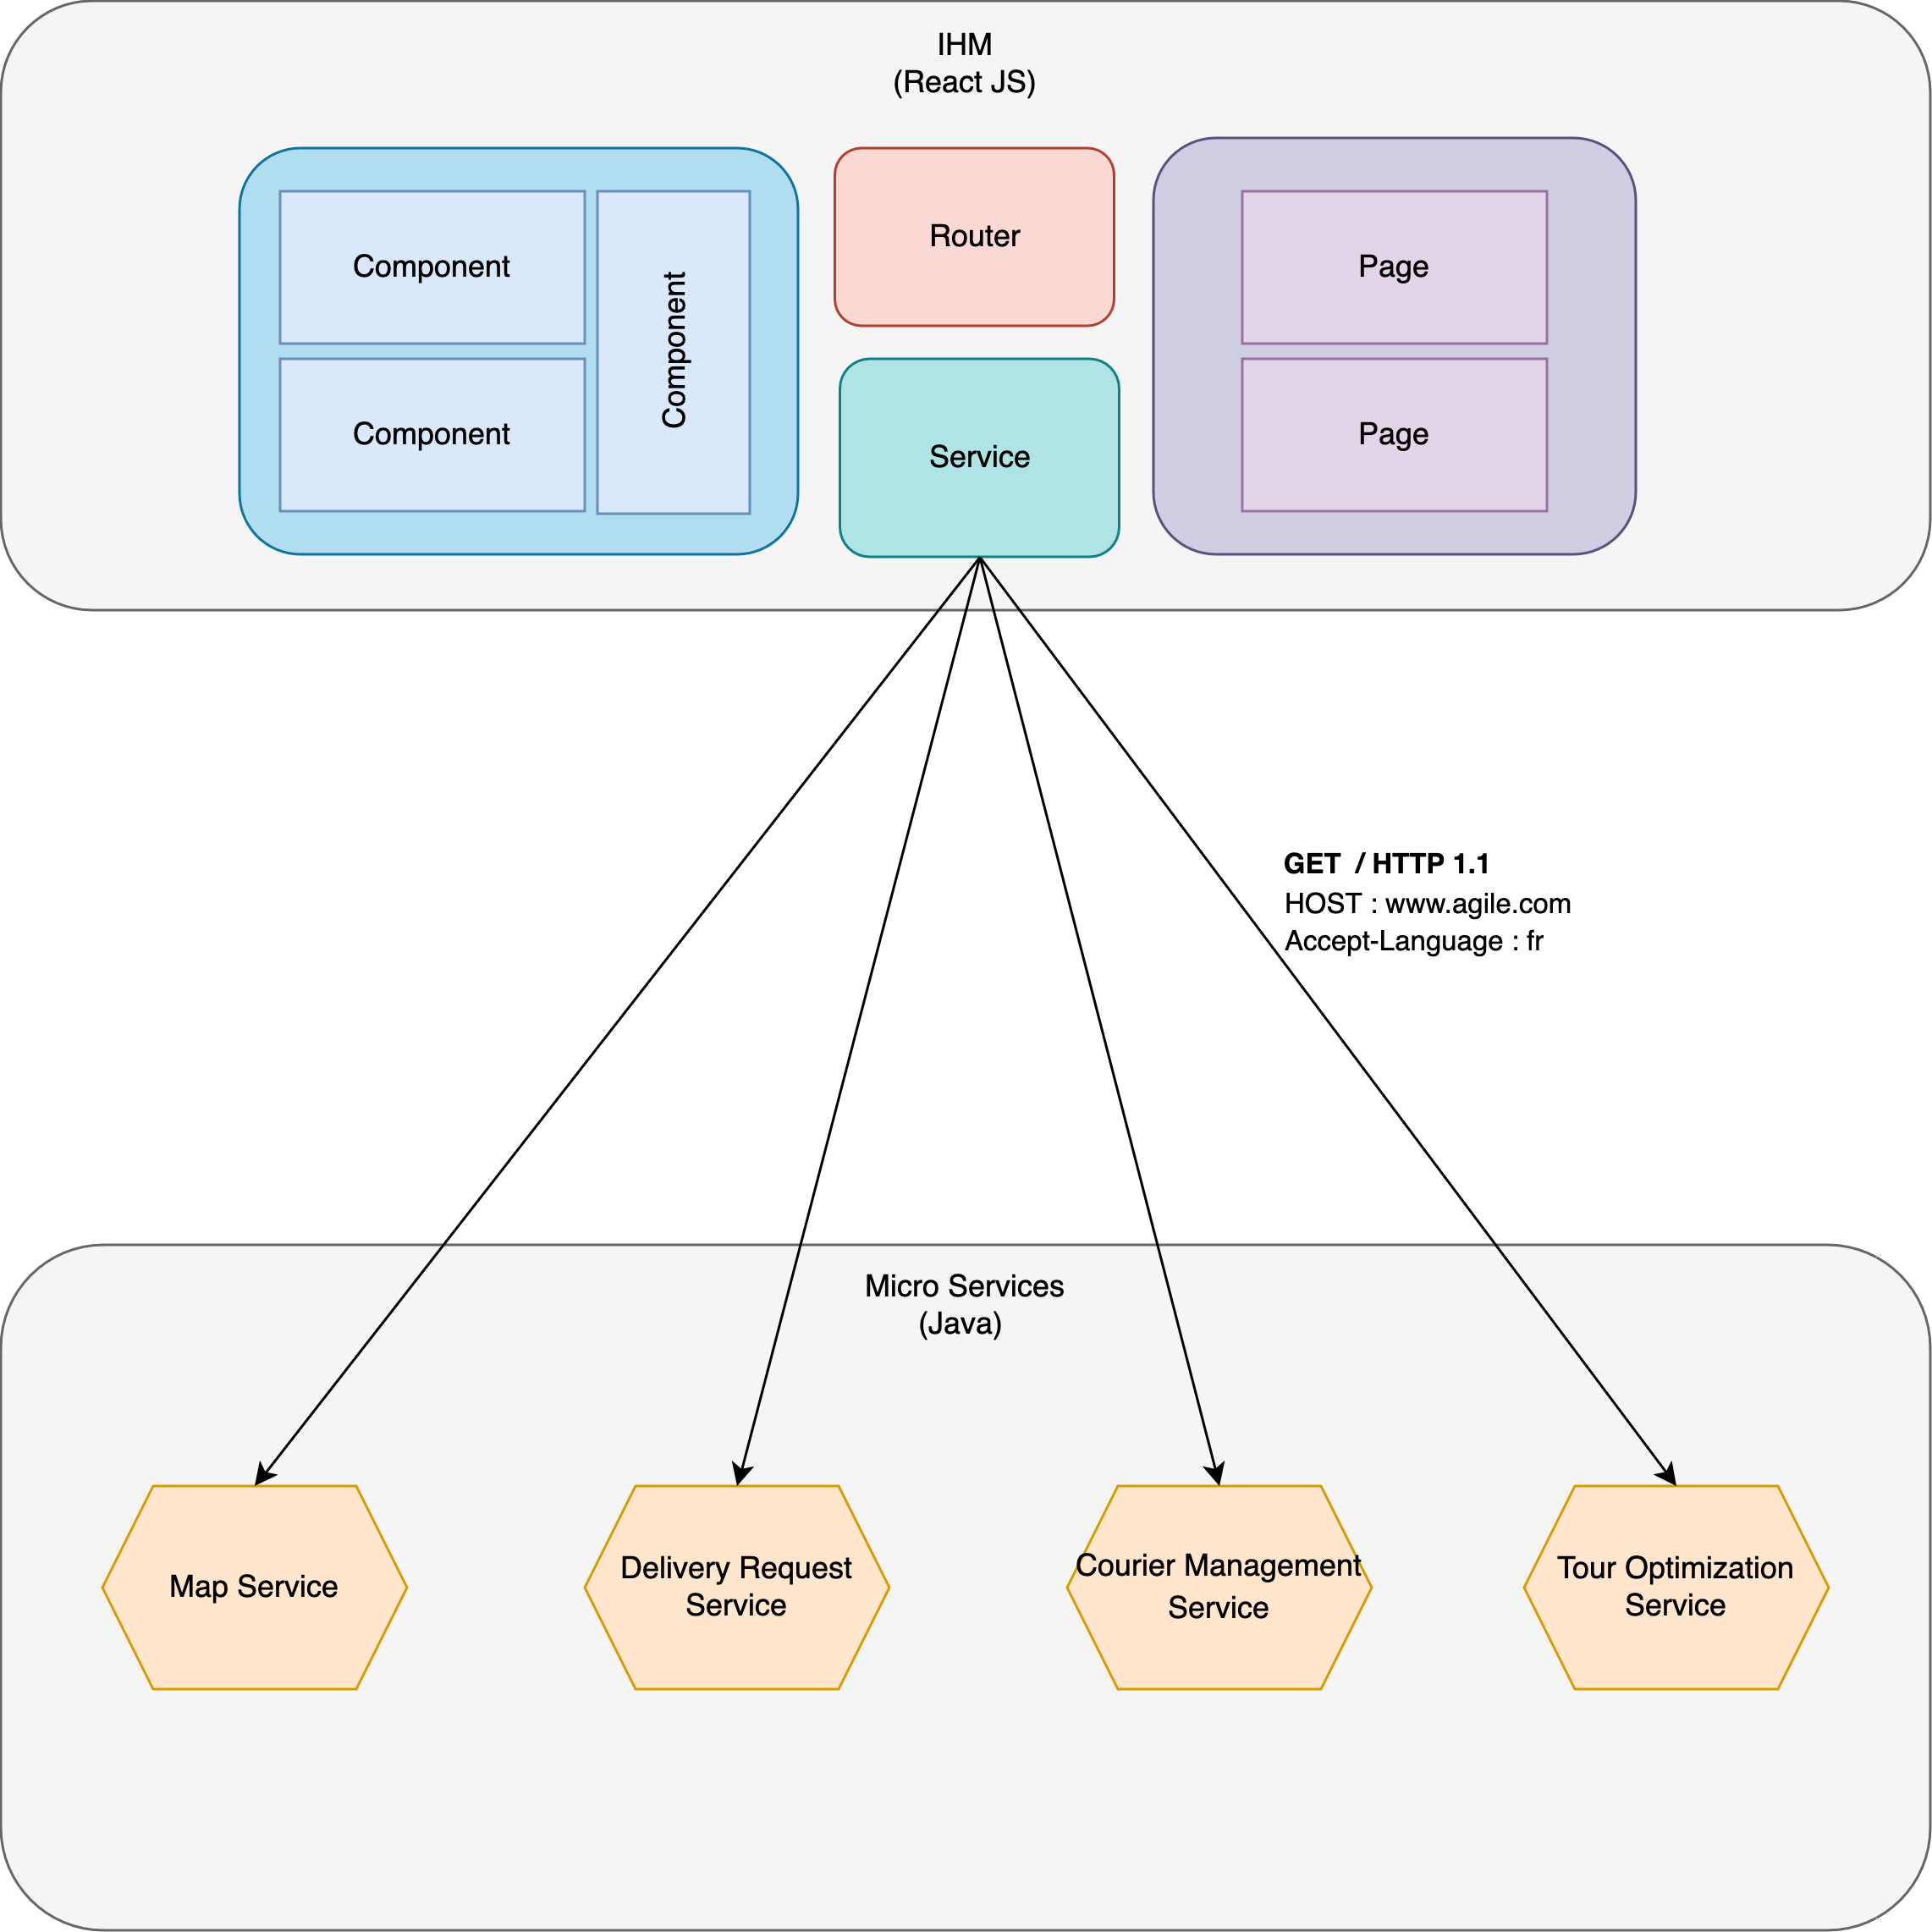
\includegraphics[width=0.75\linewidth]{images/archi.png}
\end{figure}

Notre architecture repose sur une structure en microservices, où le backend, développé en Java, est constitué de plusieurs services spécialisés : le Map Service, le Delivery Request Service, le Courier Management Service, et le Tour Optimization Service. Chaque service est indépendant et se concentre sur une fonctionnalité spécifique, ce qui garantit modularité, évolutivité et facilité de maintenance. \\

Le frontend, développé en ReactJS, suit une approche modulaire avec des composants, pages, et un routeur pour gérer la navigation. Le lien entre le frontend et le backend est assuré par un système d’API REST, qui permet une communication standardisée à travers des requêtes HTTP. Les services exposent des endpoints pour échanger des données avec le frontend, par exemple via des requêtes GET, en utilisant des protocoles courants comme HTTP 1.1. \\

Cette séparation claire entre le frontend et le backend, et l'utilisation d'API pour leur interaction, garantit la flexibilité de l'application et facilite l'intégration de nouvelles fonctionnalités ou services dans le futur.


\section{Planning}

\begin{figure}[H]
    \centering
    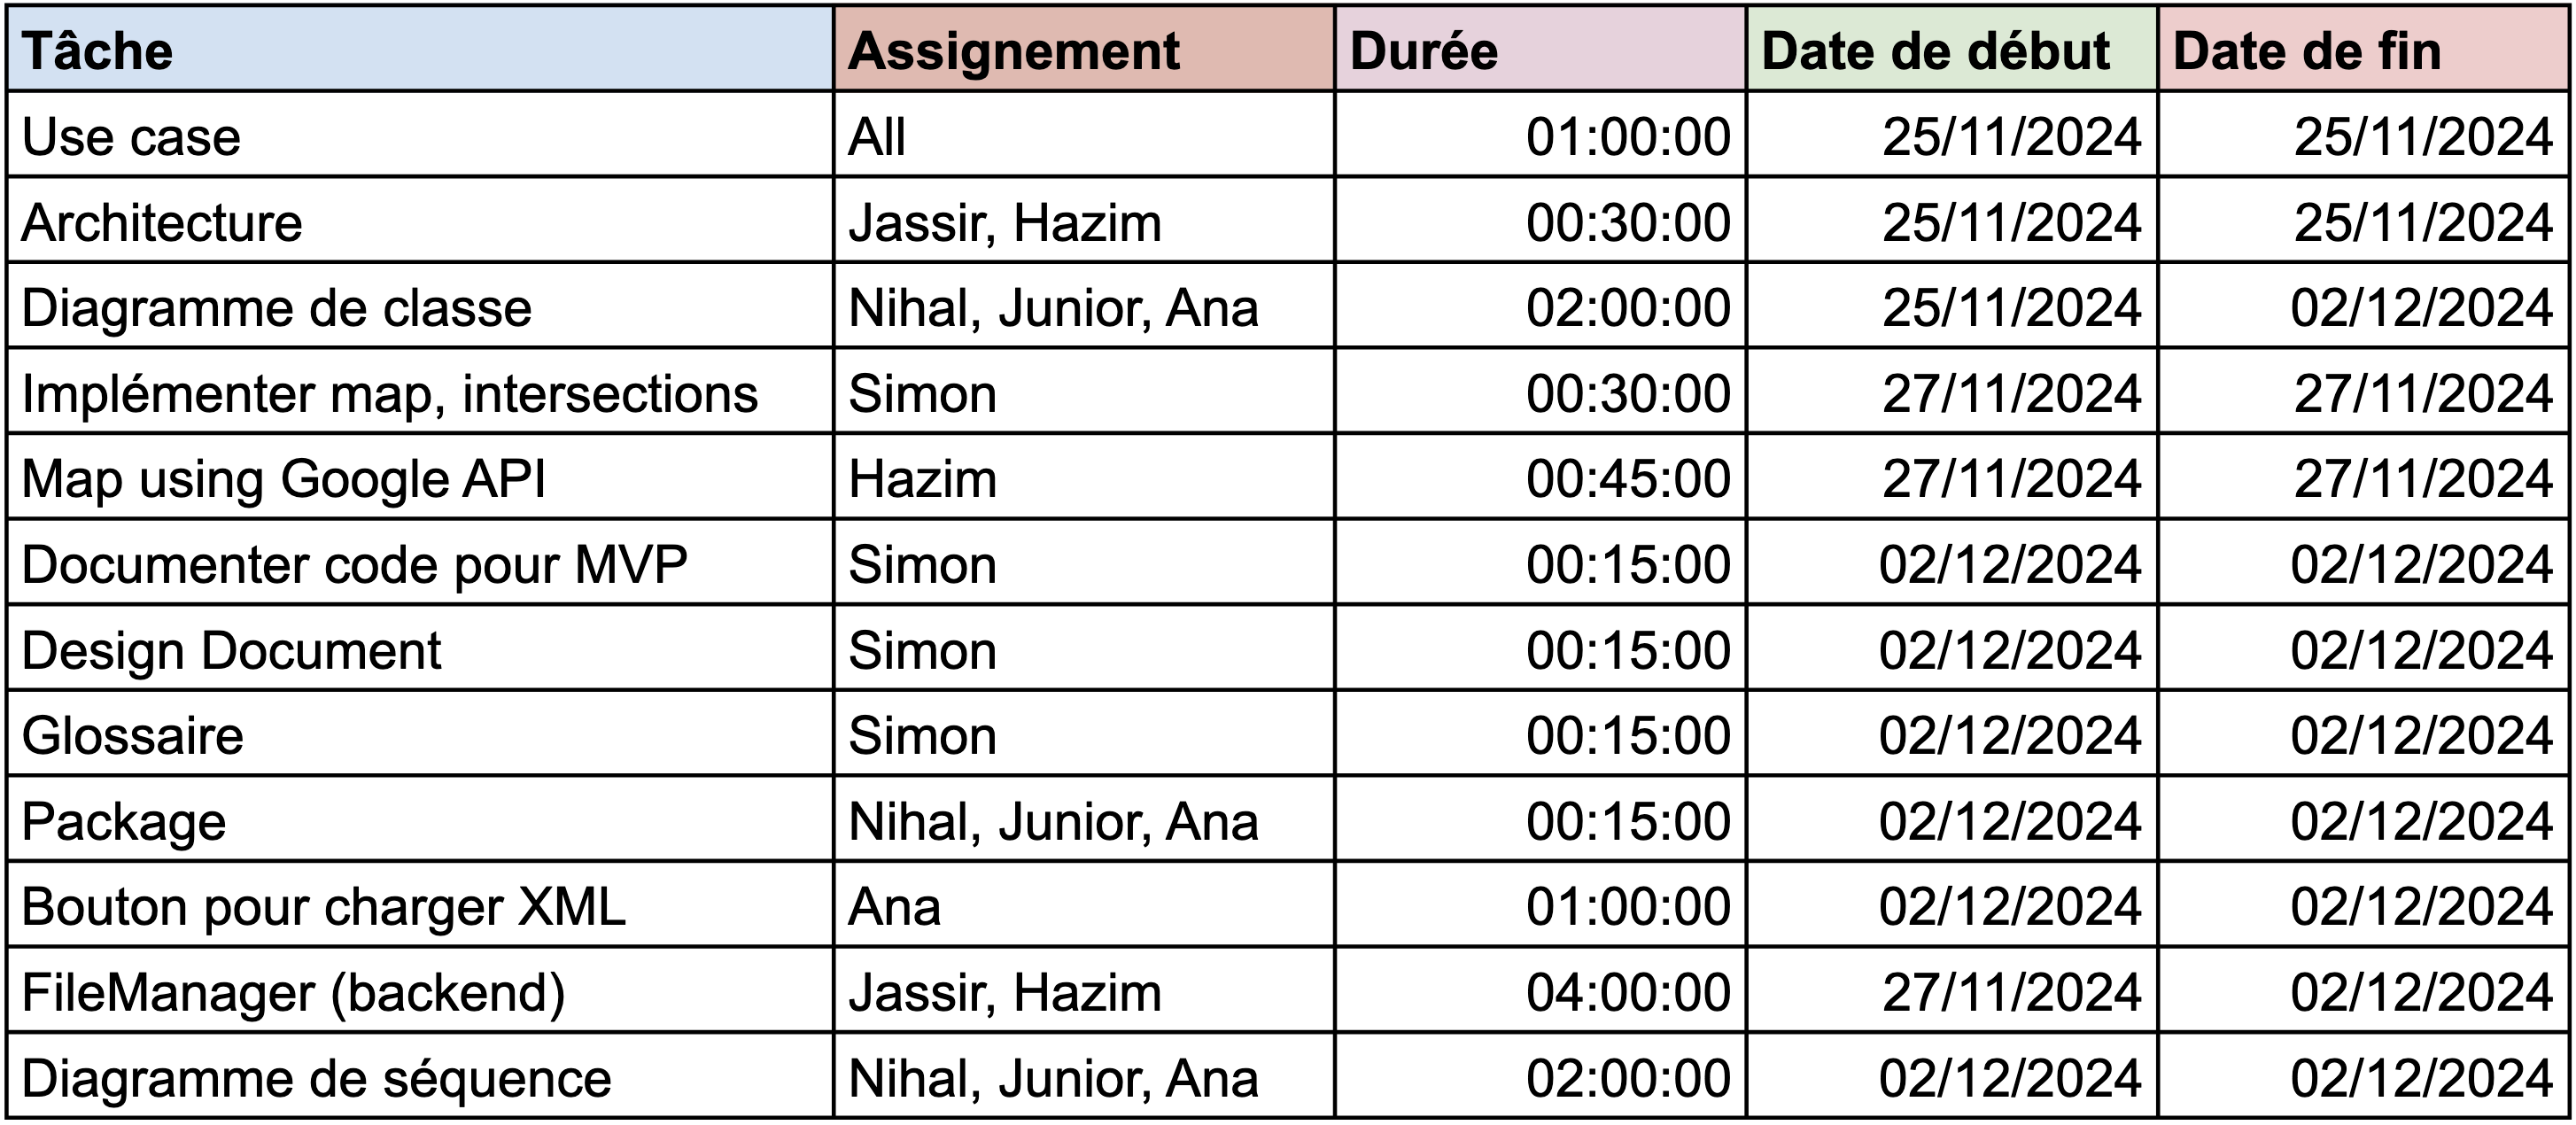
\includegraphics[width=0.75\linewidth]{images/planning.png}
    \caption{Planning des tâches}
\end{figure}

\section*{Conclusion}
Au terme de ce premier sprint, nous avons concentré nos efforts sur la phase de conception, afin d’assurer une architecture solide et cohérente pour le développement futur de notre application. Bien que cette approche ait renforcé les fondations techniques du projet, elle a également réduit le temps disponible pour le développement, ce qui nous a empêchés de finaliser toutes les fonctionnalités initialement prévues. \\
\newline
\indent Malgré ces contraintes, nous avons réussi à produire un MVP fonctionnel permettant d’afficher une carte grâce à l’intégration de l’API Google Maps. Cette base visuelle et interactive constitue un point de départ robuste pour les prochaines itérations. Cependant, la fonctionnalité de chargement de cartes depuis un fichier XML, initialement prévue dans ce sprint, n’a pas pu être implémentée dans les délais impartis.\\
\newline
\indent Cette itération a mis en lumière l’importance d’équilibrer les phases de conception et de développement pour les prochains sprints. Elle nous a également permis d’identifier des axes d’amélioration organisationnelle. Par exemple, nous avons tous pris conscience de l’importance d’utiliser efficacement le système de gestion de version Git, ce qui a permis une meilleure collaboration en équipe. En revanche, nous avons perdu du temps en raison de tâches bloquantes, qui ont freiné les autres membres de l’équipe dans leur travail.\\
\newline
\indent Pour remédier à cela, nous prévoyons de définir des tâches plus courtes et plus simples dans les prochains sprints, afin de faciliter  des commits réguliers. Cette approche devrait améliorer notre cadence et limiter les temps d’attente.

\end{document}